%!TEX root = ../thesis.tex
%*******************************************************************************
%*********************************** First Chapter *****************************
%*******************************************************************************
%The first big part is the introduction. It may seem similar to an abstract. It pursues different goals –reader hooking, providing background information and logical transition to your own research. Here is what you need to disclose in this chapter:

%Enough background information about previous researches should be presented to make readers understand place of text in science system.
%Give an explanation concerning contents – what will be included into thesis.
%Provide readers with verbal ‘road maps’.
%Cite previous works. The citations must be related to text’s goals. Do not list everything you have read about subject.
%These sections must take three pages of paper, excluding contents and table lists.

\chapter{Introduction}  %Title of the First Chapter
%********************************** %First Section  **************************************
\begin{figure*}
\centering
\subfloat[]
{
    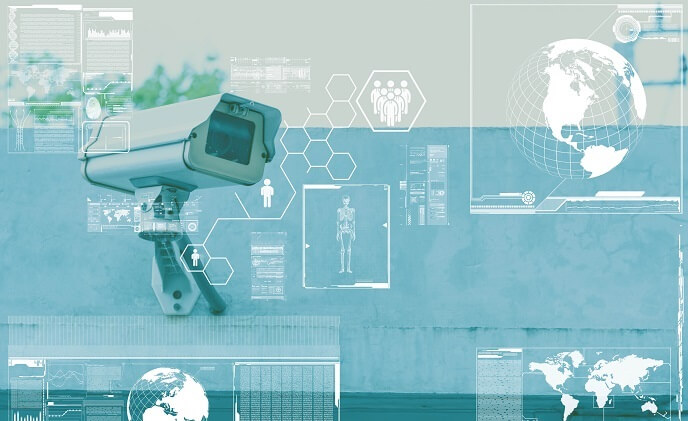
\includegraphics[scale=0.3]{Figures/cctv1.jpg}
}
\subfloat[]
{
    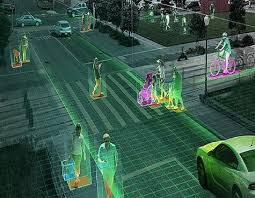
\includegraphics[scale=0.64]{Figures/cctv2.jpg}
}
\caption{Surveillance Camera Deployment and Application}
\label{fig:cctv}
\end{figure*}
Nowadays, the world is witnessing a very fast increment of camera deployment ~\citep{ananthanarayanan2019demo} as shown in Figure \ref{fig:cctv} with cities and organizations steadily increasing the size and reach of their deployments. For example, cities now deploy tens thousands of cameras, each continually collecting and streaming rich video data \cite{ref0}, \cite{ref1}, \cite{ref2}. According to IHS Markit’s annual report \cite{oliverreport}, as of 2018, “China has one camera for each 4.1 people in the country and the United State has a people-to-camera ratio of 4.6-to-1”. The massive deployments of cameras are come mainly from the growth of the video surveillance industry because of increasing the concerns about public security and safety. With this trend, the intelligent video analytics systems have been playing an essential and important role, performing main tasks in various fields including surveillance area, transportation monitoring, manufacturing, etc.
Video analytics software analyzes videos in order to detect events the system is programmed to look for – when something is moving in front of the camera.These systems analyze video sources to handle long-running tasks such as traffic monitoring, customer tracking, and surveillance. The important key to the success of such applications has been recent advances in computer vision, particularly neural network based techniques for highly accurate object detection and recognition \cite{cai2015learning}, \cite{krizhevsky2017imagenet}, \cite{li2015convolutional}.\\
In a typical real-time video analytics pipeline as 
\begin{figure*}
\centering
 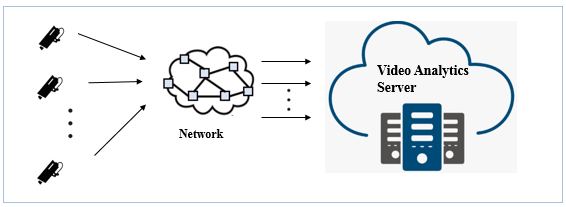
\includegraphics[width=1.0\linewidth]{Figures/cloud.png}
 \caption{Overall of cloud based video analytics server}
 \label{fig:overall}
\end{figure*}
Figure \ref{fig:overall} illustrates a traditional cloud-based video stream analytics platform. “Video analytics is performed in a a central cloud and a large number of camera transfer video data to there. However, this traditional solution makes it difficult to perform real-time video analytics on live video streams from many cameras because the VA involves several computation-consuming tasks such as object detection, object tracking, object recognition and so on. Besides, streaming video from multiple camera to the cloud consumes a lot of network bandwidth over limited-bandwidth networks, which leads to high latency, causing significant challenge for real-time video analytics” (Nguyen Van Dien and Jaehyuk Choi, 2020, p.1,2).\\
Many works has been conducted to improve the efficiency of video analytics platform \cite{canel2019scaling}, \cite{chen2015glimpse}, \cite{hsieh2018focus}, \cite{jiang2018chameleon}. Accross these systems, a typical strategy is to improve efficiency by filtering out frames that do not contain relevant information for the query using the additional edge devices. In this study, to address the question of how to address this network bottleneck and offload large volumes of data from a density camera deployment in real-time to a datacenter for further processing, we want to develope a solution by ultilizing edge computing.
“Video analytics at the edge has multiple benefits such as decreasing the response time, saving network bandwidth, and minimizing the peak workload to the cloud” (Nguyen Van Dien and Jaehyuk Choi, 2020, p.2). 
\begin{figure*}
\centering
 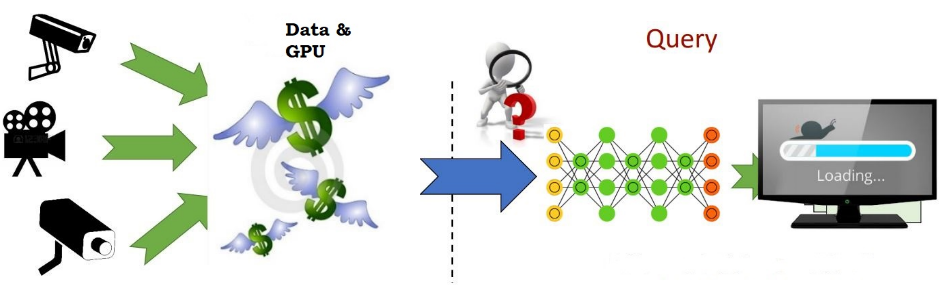
\includegraphics[width=1.0\linewidth]{Figures/vachallenge.png}
 \caption{Real-time Video Analytics Challenges}
 \label{fig:chal}
\end{figure*}
In previous works, the solutions are based on either:
\begin{itemize}
\item Binary classification model\cite{canel2019scaling}\cite{kang2017noscope}: remove frames that do not contain any object of interest.
\item Pixel-based background modeling\cite{chen2015glimpse}: eliminate frames which have not changed substantially.
\end{itemize}
Typically, exist systems use deep-learning framework to understand video frame context. Video frame is analyzed on pixel domain which require fully video decoding. However, edge devices are normally much less powerful than the cloud server, with limited computing resources such as a few CPUs, GPUs and RAM capacities \cite{stone2019towards}. In the field of public security, the ability to simultaneously process multiple camera sources and provide real-time video analytics is critical. Thus, our study seeks to overcome how edge devices and the cloud can cooperate in an efficient manner to achieve real-time and scalable video analytics. Our motivation is based on the observation that surveillance camera images are unchanged for a long time and video content is often unnecessary. So, it is undesirable to conduct analytics on redundant video frames from cameras, it will increase latency and system expense by network traffic congestion, wasting the computing resources and energy consumption in the cloud as described in Figure \ref{fig:chal}. \\
\begin{figure*}
\centering
 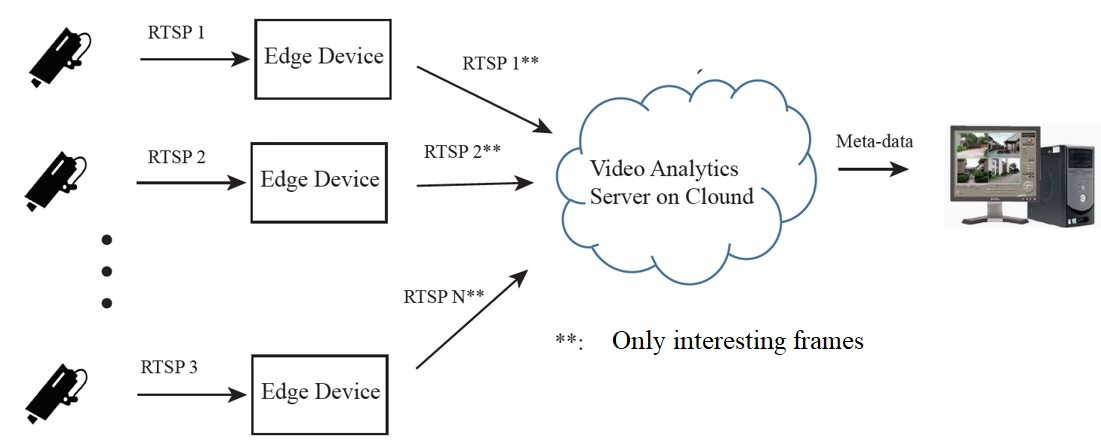
\includegraphics[width=1.0\linewidth]{Figures/motivation.jpg}
 \caption{The motivated system design}
 \label{fig:mot}
\end{figure*}
 Motivated by this pupose, we present a pre-process module that acts as a video filter function at the edge device to remove out the redundant static images before forwarding video images to the cloud for further analysis as described in Figure \ref{fig:mot}. The proposed method is driven by the compressed-domain feature which doest not require GPU-based processing and fully video decoing. Therefore, it is light-weight method and cheap solution. The  method run on an edge device and detect the motions (i.e., human walking) in the consecutive video frames. Depend on the motion detection result, the edge device decides whether to forward the video frame to the cloud or filter it out. As a result, the proposed filtering edge device can decrease not only computing resource of the cloud server but also reducing network traffic congestion to the cloud. \\
Motion detection solutions can be devided into two categories: (i) video pixel-domain based and (ii) video compressed-domain based approaches. In pixel-domain based approaches \cite{lu2014moving}, \cite{kumar2016segmentation}, \cite{gujrathi2014detecting}, \cite{wang2019ground} video is completely decoded and then applying background modelling or CNN based deep learning framework to detect moving objects at the pixel level. “The performance of video pixel-domain processing in large systems may be very challenged by the computing load of decoding multiple streams and the image pixel-based calculation. Therefores, pixel-based solution requires higher computational complexity and can make it difficult to fulfill the real-time requirement of edge devices”(Nguyen Van Dien and Jaehyuk Choi, 2020, p.2). 
Compressed-domain approaches \cite{favalli2000object},\cite{yoneyama1999moving},\cite{dong2006object},\cite{achanta2002compressed} rely on video coding artifacts of compressed bitstreams such as motion vector (MV), macroblock partitions, and quantization coefficients for recognizing motion. “Compared to pixel-domain based algorithms, compressed-domain methods generally require less computational resources because analyzing input information is already possible in the bitstream ”(Nguyen Van Dien and Jaehyuk Choi, 2020, p.2). 
\\ In this dissertation, “we proposed a compressed-domain based moving objects detection method that applies a pixel clustering and an intersection of union (IoU) score-based object tracking technique of computer vision. Using only the MVs provided by video encoders in a compressed bitstream, our approach can efficiently detect moving objects. Furthermore, an experimental evaluation of our method is provided to compare it with the state-of-the-art compressed-domain tracking methods in term of processing time, and demonstrate its functionalities to evaluate the efficiency of the proposed edge device with a cloud video analytics server in a real-world scenario. In summary, this study makes the following contributions.
\begin{itemize}
\item Utilizing Video Coding Motion Vectors (MV) analysis to filter out the static frames from video stream.
\item Present a compressed-domain based the moving objects detection method that is applied for many different surveillance applications.
\item Deploy a novel edge-to-cloud computing system for surveillance video analytics that applies the proposed method at edge devices to minimize the data transfer from surveillance camera feeds to the cloud.
\item Implementation and evaluation of the proposed method on cheap edge device (Pi4 ) and achieve real-time processing time of  39 ms/frame with high definition resolution video”(Nguyen Van Dien and Jaehyuk Choi, 2020, p.2). 
\end{itemize}
%
\nomenclature[z-VMS]{VMS}{Video Management Software}
\nomenclature[z-VA]{VA}{Video Analytics}
\nomenclature[z-CCTV]{CCTV}{Closed Circuit Television}
\nomenclature[z-CNN]{CNN}{Convolutional Neural Networks}
\nomenclature[z-FPS]{FPS}{Frames Per Second}
\nomenclature[z-MV]{MV}{Motion Vector}
\nomenclature[z-AVC]{AVC}{Advanced Video Coding}
\nomenclature[z-RTSP]{RTSP}{Real-Time Streaming Protocol}
\nomenclature[z-MCP]{MCP}{Motion-Compensated Prediction}
\nomenclature[z-HEVC]{HEVC}{High Efficiency Video Coding}
\nomenclature[z-R-CNN]{R-CNN}{Regions with CNN}
\nomenclature[z-SSD]{SSD}{Single Shot Multi-box Detector}
\nomenclature[z-YOLO]{YOLO}{You Only Look Once}
\nomenclature[z-CPU]{CPU}{Central Processing Unit}
\nomenclature[z-GPU]{GPU}{Graphics Processing Unit}
\nomenclature[z-RAM]{RAM}{Random Access Memory}
\nomenclature[z-CUDA]{CUDA}{Compute Unified Device Architecture}
\nomenclature[z-IOU]{IoU}{Intersection Over Union}
%
